
%% bare_conf_compsoc.tex
%% V1.4a
%% 2014/09/17
%% by Michael Shell
%% See:
%% http://www.michaelshell.org/
%% for current contact information.
%%
%% This is a skeleton file demonstrating the use of IEEEtran.cls
%% (requires IEEEtran.cls version 1.8s or later) with an IEEE Computer
%% Society conference paper.
%%
%% Support sites:
%% http://www.michaelshell.org/tex/ieeetran/
%% http://www.ctan.org/tex-archive/macros/latex/contrib/IEEEtran/
%% and
%% http://www.ieee.org/

%%*************************************************************************
%% Legal Notice:
%% This code is offered as-is without any warranty either expressed or
%% implied; without even the implied warranty of MERCHANTABILITY or
%% FITNESS FOR A PARTICULAR PURPOSE! 
%% User assumes all risk.
%% In no event shall IEEE or any contributor to this code be liable for
%% any damages or losses, including, but not limited to, incidental,
%% consequential, or any other damages, resulting from the use or misuse
%% of any information contained here.
%%
%% All comments are the opinions of their respective authors and are not
%% necessarily endorsed by the IEEE.
%%
%% This work is distributed under the LaTeX Project Public License (LPPL)
%% ( http://www.latex-project.org/ ) version 1.3, and may be freely used,
%% distributed and modified. A copy of the LPPL, version 1.3, is included
%% in the base LaTeX documentation of all distributions of LaTeX released
%% 2003/12/01 or later.
%% Retain all contribution notices and credits.
%% ** Modified files should be clearly indicated as such, including  **
%% ** renaming them and changing author support contact information. **
%%
%% File list of work: IEEEtran.cls, IEEEtran_HOWTO.pdf, bare_adv.tex,
%%                    bare_conf.tex, bare_jrnl.tex, bare_conf_compsoc.tex,
%%                    bare_jrnl_compsoc.tex, bare_jrnl_transmag.tex
%%*************************************************************************


% *** Authors should verify (and, if needed, correct) their LaTeX system  ***
% *** with the testflow diagnostic prior to trusting their LaTeX platform ***
% *** with production work. IEEE's font choices and paper sizes can       ***
% *** trigger bugs that do not appear when using other class files.       ***                          ***
% The testflow support page is at:
% http://www.michaelshell.org/tex/testflow/



\documentclass[conference,compsoc]{IEEEtran}
% Some/most Computer Society conferences require the compsoc mode option,
% but others may want the standard conference format.
%
% If IEEEtran.cls has not been installed into the LaTeX system files,
% manually specify the path to it like:
% \documentclass[conference,compsoc]{../sty/IEEEtran}



\usepackage{pgfplots}
\usepackage{booktabs}

% Some very useful LaTeX packages include:
% (uncomment the ones you want to load)


% *** MISC UTILITY PACKAGES ***
%
%\usepackage{ifpdf}
% Heiko Oberdiek's ifpdf.sty is very useful if you need conditional
% compilation based on whether the output is pdf or dvi.
% usage:
% \ifpdf
%   % pdf code
% \else
%   % dvi code
% \fi
% The latest version of ifpdf.sty can be obtained from:
% http://www.ctan.org/tex-archive/macros/latex/contrib/oberdiek/
% Also, note that IEEEtran.cls V1.7 and later provides a builtin
% \ifCLASSINFOpdf conditional that works the same way.
% When switching from latex to pdflatex and vice-versa, the compiler may
% have to be run twice to clear warning/error messages.






% *** CITATION PACKAGES ***
%
\ifCLASSOPTIONcompsoc
  % IEEE Computer Society needs nocompress option
  % requires cite.sty v4.0 or later (November 2003)
  \usepackage[nocompress]{cite}
\else
  % normal IEEE
  \usepackage{cite}
\fi
% cite.sty was written by Donald Arseneau
% V1.6 and later of IEEEtran pre-defines the format of the cite.sty package
% \cite{} output to follow that of IEEE. Loading the cite package will
% result in citation numbers being automatically sorted and properly
% "compressed/ranged". e.g., [1], [9], [2], [7], [5], [6] without using
% cite.sty will become [1], [2], [5]--[7], [9] using cite.sty. cite.sty's
% \cite will automatically add leading space, if needed. Use cite.sty's
% noadjust option (cite.sty V3.8 and later) if you want to turn this off
% such as if a citation ever needs to be enclosed in parenthesis.
% cite.sty is already installed on most LaTeX systems. Be sure and use
% version 5.0 (2009-03-20) and later if using hyperref.sty.
% The latest version can be obtained at:
% http://www.ctan.org/tex-archive/macros/latex/contrib/cite/
% The documentation is contained in the cite.sty file itself.
%
% Note that some packages require special options to format as the Computer
% Society requires. In particular, Computer Society  papers do not use
% compressed citation ranges as is done in typical IEEE papers
% (e.g., [1]-[4]). Instead, they list every citation separately in order
% (e.g., [1], [2], [3], [4]). To get the latter we need to load the cite
% package with the nocompress option which is supported by cite.sty v4.0
% and later.





% *** GRAPHICS RELATED PACKAGES ***
%
\ifCLASSINFOpdf
  % \usepackage[pdftex]{graphicx}
  % declare the path(s) where your graphic files are
  % \graphicspath{{../pdf/}{../jpeg/}}
  % and their extensions so you won't have to specify these with
  % every instance of \includegraphics
  % \DeclareGraphicsExtensions{.pdf,.jpeg,.png}
\else
  % or other class option (dvipsone, dvipdf, if not using dvips). graphicx
  % will default to the driver specified in the system graphics.cfg if no
  % driver is specified.
  % \usepackage[dvips]{graphicx}
  % declare the path(s) where your graphic files are
  % \graphicspath{{../eps/}}
  % and their extensions so you won't have to specify these with
  % every instance of \includegraphics
  % \DeclareGraphicsExtensions{.eps}
\fi
% graphicx was written by David Carlisle and Sebastian Rahtz. It is
% required if you want graphics, photos, etc. graphicx.sty is already
% installed on most LaTeX systems. The latest version and documentation
% can be obtained at: 
% http://www.ctan.org/tex-archive/macros/latex/required/graphics/
% Another good source of documentation is "Using Imported Graphics in
% LaTeX2e" by Keith Reckdahl which can be found at:
% http://www.ctan.org/tex-archive/info/epslatex/
%
% latex, and pdflatex in dvi mode, support graphics in encapsulated
% postscript (.eps) format. pdflatex in pdf mode supports graphics
% in .pdf, .jpeg, .png and .mps (metapost) formats. Users should ensure
% that all non-photo figures use a vector format (.eps, .pdf, .mps) and
% not a bitmapped formats (.jpeg, .png). IEEE frowns on bitmapped formats
% which can result in "jaggedy"/blurry rendering of lines and letters as
% well as large increases in file sizes.
%
% You can find documentation about the pdfTeX application at:
% http://www.tug.org/applications/pdftex





% *** MATH PACKAGES ***
%
%\usepackage[cmex10]{amsmath}
% A popular package from the American Mathematical Society that provides
% many useful and powerful commands for dealing with mathematics. If using
% it, be sure to load this package with the cmex10 option to ensure that
% only type 1 fonts will utilized at all point sizes. Without this option,
% it is possible that some math symbols, particularly those within
% footnotes, will be rendered in bitmap form which will result in a
% document that can not be IEEE Xplore compliant!
%
% Also, note that the amsmath package sets \interdisplaylinepenalty to 10000
% thus preventing page breaks from occurring within multiline equations. Use:
%\interdisplaylinepenalty=2500
% after loading amsmath to restore such page breaks as IEEEtran.cls normally
% does. amsmath.sty is already installed on most LaTeX systems. The latest
% version and documentation can be obtained at:
% http://www.ctan.org/tex-archive/macros/latex/required/amslatex/math/





% *** SPECIALIZED LIST PACKAGES ***
%
%\usepackage{algorithmic}
% algorithmic.sty was written by Peter Williams and Rogerio Brito.
% This package provides an algorithmic environment fo describing algorithms.
% You can use the algorithmic environment in-text or within a figure
% environment to provide for a floating algorithm. Do NOT use the algorithm
% floating environment provided by algorithm.sty (by the same authors) or
% algorithm2e.sty (by Christophe Fiorio) as IEEE does not use dedicated
% algorithm float types and packages that provide these will not provide
% correct IEEE style captions. The latest version and documentation of
% algorithmic.sty can be obtained at:
% http://www.ctan.org/tex-archive/macros/latex/contrib/algorithms/
% There is also a support site at:
% http://algorithms.berlios.de/index.html
% Also of interest may be the (relatively newer and more customizable)
% algorithmicx.sty package by Szasz Janos:
% http://www.ctan.org/tex-archive/macros/latex/contrib/algorithmicx/




% *** ALIGNMENT PACKAGES ***
%
%\usepackage{array}
% Frank Mittelbach's and David Carlisle's array.sty patches and improves
% the standard LaTeX2e array and tabular environments to provide better
% appearance and additional user controls. As the default LaTeX2e table
% generation code is lacking to the point of almost being broken with
% respect to the quality of the end results, all users are strongly
% advised to use an enhanced (at the very least that provided by array.sty)
% set of table tools. array.sty is already installed on most systems. The
% latest version and documentation can be obtained at:
% http://www.ctan.org/tex-archive/macros/latex/required/tools/


% IEEEtran contains the IEEEeqnarray family of commands that can be used to
% generate multiline equations as well as matrices, tables, etc., of high
% quality.




% *** SUBFIGURE PACKAGES ***
%\ifCLASSOPTIONcompsoc
%  \usepackage[caption=false,font=footnotesize,labelfont=sf,textfont=sf]{subfig}
%\else
%  \usepackage[caption=false,font=footnotesize]{subfig}
%\fi
% subfig.sty, written by Steven Douglas Cochran, is the modern replacement
% for subfigure.sty, the latter of which is no longer maintained and is
% incompatible with some LaTeX packages including fixltx2e. However,
% subfig.sty requires and automatically loads Axel Sommerfeldt's caption.sty
% which will override IEEEtran.cls' handling of captions and this will result
% in non-IEEE style figure/table captions. To prevent this problem, be sure
% and invoke subfig.sty's "caption=false" package option (available since
% subfig.sty version 1.3, 2005/06/28) as this is will preserve IEEEtran.cls
% handling of captions.
% Note that the Computer Society format requires a sans serif font rather
% than the serif font used in traditional IEEE formatting and thus the need
% to invoke different subfig.sty package options depending on whether
% compsoc mode has been enabled.
%
% The latest version and documentation of subfig.sty can be obtained at:
% http://www.ctan.org/tex-archive/macros/latex/contrib/subfig/




% *** FLOAT PACKAGES ***
%
%\usepackage{fixltx2e}
% fixltx2e, the successor to the earlier fix2col.sty, was written by
% Frank Mittelbach and David Carlisle. This package corrects a few problems
% in the LaTeX2e kernel, the most notable of which is that in current
% LaTeX2e releases, the ordering of single and double column floats is not
% guaranteed to be preserved. Thus, an unpatched LaTeX2e can allow a
% single column figure to be placed prior to an earlier double column
% figure. The latest version and documentation can be found at:
% http://www.ctan.org/tex-archive/macros/latex/base/


%\usepackage{stfloats}
% stfloats.sty was written by Sigitas Tolusis. This package gives LaTeX2e
% the ability to do double column floats at the bottom of the page as well
% as the top. (e.g., "\begin{figure*}[!b]" is not normally possible in
% LaTeX2e). It also provides a command:
%\fnbelowfloat
% to enable the placement of footnotes below bottom floats (the standard
% LaTeX2e kernel puts them above bottom floats). This is an invasive package
% which rewrites many portions of the LaTeX2e float routines. It may not work
% with other packages that modify the LaTeX2e float routines. The latest
% version and documentation can be obtained at:
% http://www.ctan.org/tex-archive/macros/latex/contrib/sttools/
% Do not use the stfloats baselinefloat ability as IEEE does not allow
% \baselineskip to stretch. Authors submitting work to the IEEE should note
% that IEEE rarely uses double column equations and that authors should try
% to avoid such use. Do not be tempted to use the cuted.sty or midfloat.sty
% packages (also by Sigitas Tolusis) as IEEE does not format its papers in
% such ways.
% Do not attempt to use stfloats with fixltx2e as they are incompatible.
% Instead, use Morten Hogholm'a dblfloatfix which combines the features
% of both fixltx2e and stfloats:
%
% \usepackage{dblfloatfix}
% The latest version can be found at:
% http://www.ctan.org/tex-archive/macros/latex/contrib/dblfloatfix/




% *** PDF, URL AND HYPERLINK PACKAGES ***
%
%\usepackage{url}
% url.sty was written by Donald Arseneau. It provides better support for
% handling and breaking URLs. url.sty is already installed on most LaTeX
% systems. The latest version and documentation can be obtained at:
% http://www.ctan.org/tex-archive/macros/latex/contrib/url/
% Basically, \url{my_url_here}.




% *** Do not adjust lengths that control margins, column widths, etc. ***
% *** Do not use packages that alter fonts (such as pslatex).         ***
% There should be no need to do such things with IEEEtran.cls V1.6 and later.
% (Unless specifically asked to do so by the journal or conference you plan
% to submit to, of course. )


% correct bad hyphenation here
\hyphenation{op-tical net-works semi-conduc-tor}


\begin{document}
%
% paper title
% Titles are generally capitalized except for words such as a, an, and, as,
% at, but, by, for, in, nor, of, on, or, the, to and up, which are usually
% not capitalized unless they are the first or last word of the title.
% Linebreaks \\ can be used within to get better formatting as desired.
% Do not put math or special symbols in the title.
\title{Analyzing the Popularity of News Articles Using Linear Regression}

% author names and affiliations
% use a multiple column layout for up to three different
% affiliations
\author{
\IEEEauthorblockN{Jonathan Campbel}
\IEEEauthorblockA{School of Computer Science\\
	jonathan.campbell@mail.mcgill.ca}
\and
\IEEEauthorblockN{Yann Aublet-Longpré}
\IEEEauthorblockA{Department of Biology\\
yann.aublet-longpre@mail.mcgill.ca}
\and
\IEEEauthorblockN{Jian (Ethan) Li}
\IEEEauthorblockA{School of Computer Science\\
	jian.li9@mail.mcgill.ca}
}

% conference papers do not typically use \thanks and this command
% is locked out in conference mode. If really needed, such as for
% the acknowledgment of grants, issue a \IEEEoverridecommandlockouts
% after \documentclass

% for over three affiliations, or if they all won't fit within the width
% of the page (and note that there is less available width in this regard for
% compsoc conferences compared to traditional conferences), use this
% alternative format:
% 
%\author{\IEEEauthorblockN{Michael Shell\IEEEauthorrefmark{1},
%Homer Simpson\IEEEauthorrefmark{2},
%James Kirk\IEEEauthorrefmark{3}, 
%Montgomery Scott\IEEEauthorrefmark{3} and
%Eldon Tyrell\IEEEauthorrefmark{4}}
%\IEEEauthorblockA{\IEEEauthorrefmark{1}School of Electrical and Computer Engineering\\
%Georgia Institute of Technology,
%Atlanta, Georgia 30332--0250\\ Email: see http://www.michaelshell.org/contact.html}
%\IEEEauthorblockA{\IEEEauthorrefmark{2}Twentieth Century Fox, Springfield, USA\\
%Email: homer@thesimpsons.com}
%\IEEEauthorblockA{\IEEEauthorrefmark{3}Starfleet Academy, San Francisco, California 96678-2391\\
%Telephone: (800) 555--1212, Fax: (888) 555--1212}
%\IEEEauthorblockA{\IEEEauthorrefmark{4}Tyrell Inc., 123 Replicant Street, Los Angeles, California 90210--4321}}




% use for special paper notices
%\IEEEspecialpapernotice{(Invited Paper)}




% make the title area
\maketitle

% As a general rule, do not put math, special symbols or citations
% in the abstract
\begin{abstract}
We apply linear regression to two datasets of news articles, one newly-created, to predict popularity of the articles and present our findings.
\end{abstract}

% no keywords


% For peer review papers, you can put extra information on the cover
% page as needed:
% \ifCLASSOPTIONpeerreview
% \begin{center} \bfseries EDICS Category: 3-BBND \end{center}
% \fi
%
% For peerreview papers, this IEEEtran command inserts a page break and
% creates the second title. It will be ignored for other modes.
\IEEEpeerreviewmaketitle



\section{Introduction}
% no \IEEEPARstart
% tasked by newspaper ?
% mention that cbc news is the dataset
In this project, we build a machine learning (ML) system to predict the popularity of online news articles of two datasets, each with different features. Indeed, the online news platform is becoming a very important source of information. Its low cost and relative ease of distribution mean it can reach a vast audience, but it also means that there exists an intense competition for attention. The resulting asymmetry in the distribution of collective attention makes work like the present one extremely valuable to content providers, journalists and advertisers alike.

Two separate approaches have been taken to solve the problem at hand. The first method is to take data available immediately after the article publication to predict its final popularity. The second is to predict the popularity using only the information available prior to the publication. The features employed for the latter are metadata, such as topic, authors, date of publication, number of words, etc as well as semantic characteristic, like keywords or natural language processing. The First method typically make use of early click through, such as the number of comments in the first few hours.

Many different target variables can be used to express the popularity of content: the number of views, comments, shares and user votes all work well as metrics for popularity. In this project we explored two particular metrics. In Part 1, where we analyze an existing dataset of Mashable articles \cite{fernandes-2015-proactive}, the number of shares is our target variable, while in Part 2, where we analyze a new dataset of CBC News articles\footnote{The dataset is available for download at http://www.campbelljc.com/cbc.csv}, we use the number of comments.

% You must have at least 2 lines in the paragraph with the drop letter
% (should never be an issue)

\subsection{Related Work}
In related work \cite{szabo2010predicting}, Szabo and Huberman studied, using the platforms Digg and YouTube, how popularity of an online content could be predicted soon after submission. They found a linear correlation between the logarithm transform of the early and later popularity. The prediction made by their linear regression by least-squared error displayed a lot of variance, while minimizing over relative errors displayed considerably smaller dispersion. Consequently, they favored the relative error model.

Similarly, Tatar et al. \cite{tatar2011predicting} showed how a simple linear regression model could help to predict the volume of comments from an online news article based on the number of comments observed within a certain period after publication.

Next, Tsagkias et al. \cite{tsagkias2009predicting} presented an exploratory work on predicting the volume of comments in news articles prior to publication. They looked at datasets for many sources and addressed the prediction task as one of classification.

Bandari et al. \cite{bandari2012pulse} worked on predicting the popularity of news items on Twitter using features extracted prior to the article release. Their results show that these features might not be sufficient to predict the exact number of tweets, but can be effective at a similar classification task.
% which similar task ?

Finally, Fernandes et al. \cite{fernandes-2015-proactive} explored the same dataset that we used for Part 1 and implemented five different classifier models to first predict which articles would become popular and then optimize a subset of the features to enhance the predicted popularity. 

\subsection{Outline} 
In the present work, we applied linear regression on a set of features to predict a target variable which represents popularity. We applied our algorithm to two separate datasets: the first one containing Mashable articles taken from the UCI Machine Learning repository articles, and the second containing articles from CBC News which were gathered by a web crawler.

This paper is divided as follows: first, we present our datasets, and describe how they were acquired and processed. Then, we introduce linear regression and show how the method of least-squares can be solved both in closed-form and using gradient descent. Next, we expose our experimental results. We conclude with a brief discussion of the usefulness of the project, offering future ideas for dataset acquisition.  

\section{Methods}

\subsection{Data Acquisition and Preparation}

\subsubsection{Part 1}

For the first part of our project, we used a dataset consisting of Mashable articles prepared by Fernandes et al. \cite{fernandes-2015-proactive} from the UCI Machine Learning repository \cite{lichman-2013-ucimlrepo}. The dataset consists of 39,797 articles published over a period of two years. There are 58 predictive features, all of which are obtained prior to publication of an article. These features can be broken down into seven categories: words, links, digital media, time, keyword and natural language processing. The target variable is the number of shares.

The only transformation that we did on the features was to normalize them, which must be done in order to apply ridge regularization. As we have seen in class, this linear transformation does not affect the decision boundary. All features are scaled and restricted to be between $-1$ and $1$. Apart from this, no feature recoding was done since it was not allowed in this part of the project. Further, we chose not to drop any of the features present in the database, even though we noticed quite a bit of redundancy in the data. 

Finally, training and testing data were split in pre-processing, that is, after the data was randomized to discard any latent pattern in the dataset. $80\%$ of the original data was allocated to the training set while $20\%$ was kept in the testing set for evaluation.

\begin{table}[]
	\centering
	\caption{Statistical Measure for the Training set}
	\label{table1}
	\begin{tabular}{@{}ll@{}}
		Number of Articles                      & 31,715                       \\
		Average Number of Shares                & 3,424                        \\
		Maximum Number of Shares                & 1                           \\
		Minimum Number of Shares                & 843,300                      \\
		Standard Deviation                      & 12,323
	\end{tabular}
\end{table}

\subsubsection{Part 2}

The CBC News website was chosen for the acquisition of our news article dataset. We based our crawler code on an open source Python project \cite{invernizzi-2013-crawler}, which has the ability to render crawled pages in a browser setting, so that the asynchronous JavaScript (AJAX) and other communication protocols (e.g. WebSocket) can execute and fetch various parts of the page. This feature is important since, on any particular CBC News article page, several parts of the page are only loaded after rendering has completed through the aforementioned methods.

The crawling code was subsequently modified from the original to conform specifically to the chosen website. In particular, the area of the Internet to crawl was limited to pages beginning with the URI \"http://www.cbc.ca/news\", the domain and directory in which the news articles reside. Furthermore, several subsections of said location were disallowed, including the Sports, Interactive, and Archives sub-sections of the site, due either to a lack of news articles in those directories or to non-conformity with established (regular) article HTML format.

When a news article is found by the crawler, metadata about the article will be extracted and placed into a new datafile. This metadata includes the URL, article category, sub-category, story flag (whether the piece is an Analysis piece, e.g.), title, description, author, post date, number of headlines within the article body, and the numbers of paragraphs, videos, links, inline images, shares, and comments. The approach to save each article's metadata within its own file was taken to preserve data in case of crawler instability (due to potential non-conforming news article HTML structure).

Any article where the crawler was unable to extract number of comments and/or number of shares was discarded. Some complete sections of the CBC site do not have comment sections (e.g. news local to Hamilton, Ontario), while other individual articles have no comment section, possibly done on purpose by the article author. Further, some articles were discarded because either comment or share sections of the site did not load in time for the crawler to save them. For purposes of time, the crawler devoted at most 10 seconds waiting for each page to load.

In total, approximately 3,000 news articles were crawled and their metadata parsed for our dataset. A further 3,500 articles were crawled and discarded due to the aforementioned reasons.

Another Python script takes in all article metadata, and does further processing on it to extract more relevant features. These features include number of words in title, number of authors, average length of words in title, number of numbers in title, whether the article was posted on a weekday or weekend, and whether it was posted in the morning, afternoon, or evening. The script also converts some numerical values to binary ones (e.g. a category of Aboriginal news would set the isAboriginal feature to 1). All features end up being represented by numerical or binary values (see Appendix 1 for a complete listing of features).

We also used a Natural Language Processing library to calculate a sentiment value for the title of each news article \cite{stanfordcorenlp}. The sentiment value of an article could be \textit{very negative} (assigned numeric value $-2$), \textit{negative} ($-1$), \textit{neutral} ($0$), \textit{positive} ($1$) and \textit{very positive} ($2$).

\subsection{Linear Regression}
Linear regression is a widely used statistical tool for modeling relationship between predictory variables $X_i$ (features) and some outcome y (target variable). In particular, we assume that our target variable y can be estimated from a linear hypothesis of the form:

\begin{equation}
f_{W}(X) = w_{0} +  \sum_{j=1}^m w_{j}X_{j}
\end{equation} 

The goal of our learner is to find the parameter vector W that minimizes the discrepancy between the predicted value $\hat{y}$ and the actual outcome y. We define the loss function to minimize as the mean squared error:

\begin{equation}
L_{s}(f) = \frac{1}{n} \sum_{i=1}^n (y_{i} - \hat{y}_{i})^2
\end{equation}

In this section, we display two algorithms that we implemented to solve this problem. We show how this can be solved first in closed-form, and second using gradient descent. Finally, we present Ridge regression and an approximated version of Lasso regression.

\subsubsection{Closed-Form}

For simplicity, let us re-write the equation (1) in matrix form:
\begin{equation}
f_{W}(X) = XW
\end{equation}
\begin{tabbing}
	where: \= $X$, the \= design matrix, is $n \times m$, with: \+\+ \\ $n$ := number of  training examples \\ $m$ := number of features \-\\
	$W$, the parameter vector, is $m \times 1$
\end{tabbing} 
Likewise for the loss function: 
\begin{equation}
L_{s}(f) = \frac{1}{n} (Y- XW)^T(Y-XW)
\end{equation}
Where Y, the target vector, is nx1

To minimize the loss funcion, we take its derivative with respect to W and equate it to zero: 
\begin{equation}\label{eq:gradient}
\frac{\partial L_{s}(f)}{\partial W} = 0 = \frac{-2}{n} X^T(Y-XW)
\end{equation} 
Solving for W, we get:
\begin{equation}
W = (X^TX)^{-1}X^TY
\end{equation}
Given that the matrix $(X^TX)$ is invertible, an exact solution to this equation can be found in closed-form. In our implementation, we use the jblas linear algebra for Java library (cite) to perform the matrix multiplications. We also implemented an algorithm to do the matrix inversion that find a matrix $X^{-1}$ that solves:
\begin{equation}
X^{-1}X = I
\end{equation} 
where I is the identity matrix.

The computation cost for this algorithm lies mostly with the matrix inversion, which can be done in polynomial time with respect to the size of the matrix $(X^TX)$. Although this can cause problem when handling very large datasets, the method performs very well for our present application.

\subsubsection{Gradient Descent}

A gradient descent approach is also implemented for this project. In the gradient descent approach, instead of looking at close form solution, we look at the gradient of the error function (equation \ref{eq:gradient}), choose a set of initial weights, and iteratively find the solution. This approach is specially useful when the data set is too large where a direct solution would not be possible.

One of the key part in the gradient descent approach is deciding the learning rate $\alpha$. A learning rate too big would result in the algorithm not descending to a minimum. In fact, in part 1, a learning rate too big will result in the weights going to infinity after a few iterations.

A simple checking mechanism was implemented to make sure that the learning rate is not too big. Before actually starting the gradient descent, we check the least square error at the starting point, and calculate the least square error after $1$ step of gradient descent. If the error gets bigger, that would mean the learning rate $\alpha$ is too big. We then scale it to a smaller value, and repeat the process until the error gets smaller after $1$ step of gradient descent.

We chose the $0$ vector as the initial weights for the gradient descent.

One important reason we implemented data normalization is because of the gradient descent approach.

In our development process, we found that when the data is not scaled, it takes a very long time for the gradient descent to run. We used the above mentioned mechanism to find the largest possible learning rate $\alpha$, and yet it has a very slow converging speed. See figure \ref{fig:withwithoutreg}.


\begin{figure}
	\centering
	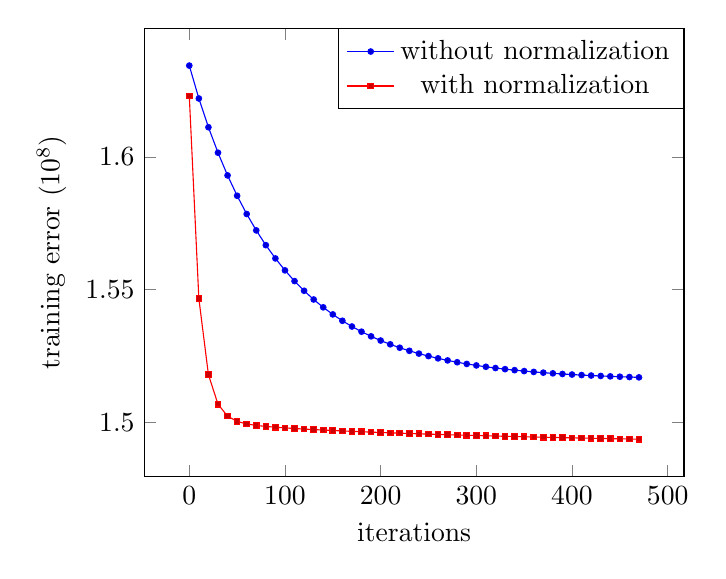
\begin{tikzpicture}
	\begin{axis}
	[
	mark size=1pt,
	legend style={at={(1,1)},anchor=north east},
	xlabel={iterations},
	ylabel={training error ($10^8$)}
	]
	\addplot coordinates
	{
	(0, 1.6344811780988837)
	(10, 1.6220757736685407)
	(20, 1.611230509164933)
	(30, 1.601628549527569)
	(40, 1.593065828171678)
	(50, 1.5853987502656735)
	(60, 1.5785178976490986)
	(70, 1.5723346137120666)
	(80, 1.5667739885169074)
	(90, 1.5617710422887463)
	(100, 1.5572685232525842)
	(110, 1.553215534511018)
	(120, 1.5495665991462206)
	(130, 1.546280967725429)
	(140, 1.5433220689098264)
	(150, 1.540657051770987)
	(160, 1.5382563922998187)
	(170, 1.536093548600194)
	(180, 1.5341446553806748)
	(190, 1.5323882515567782)
	(200, 1.530805036514089)
	(210, 1.5293776515824438)
	(220, 1.528090483894029)
	(230, 1.5269294902194217)
	(240, 1.525882038687654)
	(250, 1.5249367665418383)
	(260, 1.5240834522874784)
	(270, 1.5233129007649016)
	(280, 1.5226168398320983)
	(290, 1.5219878274790046)
	(300, 1.521419168315411)
	(310, 1.5209048384835206)
	(320, 1.5204394181418048)
	(330, 1.5200180307544586)
	(340, 1.5196362884980654)
	(350, 1.5192902431675028)
	(360, 1.5189763420252758)
	(370, 1.5186913880950186)
	(380, 1.5184325044509581)
	(390, 1.5181971020996008)
	(400, 1.5179828510917706)
	(410, 1.5177876545389566)
	(420, 1.5176096252415032)
	(430, 1.5174470646653602)
	(440, 1.5172984440306845)
	(450, 1.517162387300016)
	(460, 1.5170376558744887)
	(470, 1.5169231348263152)
	};
	\addlegendentry{without normalization}
	\addplot coordinates
	{
	(0, 1.6230459226869196)
	(10, 1.5466157111394947)
	(20, 1.5179464415115493)
	(30, 1.5068021505521172)
	(40, 1.5022841550969048)
	(50, 1.5003180042284747)
	(60, 1.4993547786724135)
	(70, 1.4987987644274605)
	(80, 1.4984176658304498)
	(90, 1.498118905131215)
	(100, 1.4978641960384276)
	(110, 1.4976367038271723)
	(120, 1.4974283081239765)
	(130, 1.4972345947160837)
	(140, 1.4970528423877514)
	(150, 1.4968811840529295)
	(160, 1.496718236846958)
	(170, 1.496562925046218)
	(180, 1.4964143859810772)
	(190, 1.4962719141698018)
	(200, 1.4961349247216735)
	(210, 1.496002927525644)
	(220, 1.4958755081214024)
	(230, 1.4957523130723327)
	(240, 1.4956330385594439)
	(250, 1.4955174213739293)
	(260, 1.4954052317419673)
	(270, 1.4952962675724062)
	(280, 1.4951903498212606)
	(290, 1.4950873187396228)
	(300, 1.4949870308244149)
	(310, 1.4948893563303587)
	(320, 1.494794177232557)
	(330, 1.4947013855513727)
	(340, 1.4946108819700483)
	(350, 1.4945225746889266)
	(360, 1.4944363784725223)
	(370, 1.494352213852695)
	(380, 1.4942700064602354)
	(390, 1.4941896864609738)
	(400, 1.4941111880779583)
	(410, 1.494034449184753)
	(420, 1.4939594109571603)
	(430, 1.493886017573658)
	(440, 1.4938142159565002)
	(450, 1.4937439555462075)
	(460, 1.4936751881048498)
	(470, 1.4936078675428748)
	};
	\addlegendentry{with normalization}
	\end{axis}
	\end{tikzpicture}
	\caption{Gradient Descent: converging speed with and without regularization}\label{fig:withwithoutreg}
\end{figure}


\subsubsection{Ridge Regression}

The solution given by the least-squares estimate is unbiased. In fact, we know from the Gauss-Markov Theorem that the least-squares estimate gives the best unbiased linear estimate, meaning that it has the smallest variance amongst all unbiased estimates. However, in some case it is better to add a little biasness in favor of a smaller variance. This can happen if the features are highly correlated. Ridge Regression or Tikhonov regularization can be used to alleviate multicollinearity amongst features. Mathematically, this is implemented by adding a second term to equation (2)
\begin{equation}
L_{s}(f) = \frac{1}{n} \sum_{i=1}^n (y_{i} - \hat{y}_{i})^2 + \lambda \sum_{j=1}^m w_{j}^2
\end{equation}

In essence, what this does is to prevent over-fitting by imposing a penalty on the model size, as characterized by the second term. The rest of the algorithm is similar to what we described in section 2.2.1, we minimize the loss function by taking its derivative with respect to W. Solving for W in $\frac{\partial L_{s}(f)}{\partial W} = 0$ we get:
\begin{equation}
W = (X^TX+\lambda I)^{-1}X^TY
\end{equation}

Which can be solved directly by the numerical machinery we set up in 2.2.1 or via gradient descent, as in 2.2.2. This solution shrinks the weight down, effectively reducing the model complexity, it is said to give a smooth solution. Note that the ridge regression is not invariant under scaling, which is why we normalized our data during pre-processing.


\subsubsection{Lasso Regression} While Ridge regression gives a smooth solution, a more sparse solution could be preferred in certain scenarios. Lasso regression is more suitable for these situations \cite{tibshirani1996regression}. 
Different from Ridge regression, the Lasso uses $L1$ regularization:

\begin{equation}\label{eq:lasso}
L_{s}(f) = \frac{1}{n} \sum_{i=1}^n (y_{i} - \hat{y}_{i})^2 + \lambda \sum_{j=1}^m |w_{j}|
\end{equation}

Ridge regression effectively shrinking the weights, but drives few weights to 0. The Lasso, on the other hand, has the property that if $\lambda$ is sufficiently large, some of the coefficients $w_j$ are driven to zero \cite{bishop2006pattern}.

There is no close-form solution for Lasso regression and the implementation is harder than Ridge regression, and also more computationally expensive.

An approximated approach was presented in \cite{fan2001variable}. The approach was based on the following approximation:

\begin{equation}
	|w_i|_1 \approx \frac{{w_i}^2}{|w_i|}_1
\end{equation}

Plug it into equation \ref{eq:lasso}, we can derive an iterative updating scheme:
\begin{equation}
w_{new} = (X^T X + \lambda diag(|w_{old}|)^{-1} )^{-1} X^T Y
\end{equation}

There are some problems with this approach, such as that once one feature is driven to $0$, it will never be driven away from $0$, and that it sometimes gets suboptimal results instead of the optimal result. However, we chose to implement this approach because implementation for this approach is very simple and it is not very computationally expensive \cite{fan2001variable}.

Lasso regression can be used for feature selection.

\section{Implementation}

The linear regression algorithm is implemented through Java. The library \textit{OpenCSV} \cite{opencsv} is used in this project to load and parse dataset files. The linear algebra library \textit{jblas} \cite{jblas} is used for matrix computation.

The web crawler was implemented with Python, and uses an open source Python project \cite{invernizzi-2013-crawler}. 

For part 2, we also used a Natural Language Processing library, Stanford CoreNLP \cite{stanfordcorenlp}, to calculate the sentiment of new titles.

\section{Results}

\subsection{Part 1}

\begin{table}[]
	\centering
	\caption{Training and Test Errors for Part 1}\label{table:part1results}
	\begin{tabular}{lll}
		& Training Error                            & Test Error           \\
		Close Form                & $1.48485 \times 10^8$ & $6.6537 \times 10^7$ \\
		Close Form (Ridge)        & $1.48488 \times 10^8$ & $6.6548 \times 10^7$ \\
		Gradient Descent          & $1.49116 \times 10^8$ & $6.6871 \times 10^7$ \\
		Gradient Descent (Ridge)  & $1.49117 \times 10^8$ & $6.6871 \times 10^7$ \\
		Lasso (Approximation)  & $1.48485 \times 10^8$ & $6.6537 \times 10^7$  \\       
	\end{tabular}
\end{table}

The training and testing errors of different approaches tried in this project is listed in table \ref{table:part1results}. The epsilon value for gradient descent was set to 5.0.

As can be seen in the table, for our training and test data split, the test error is much smaller than the training error. However, in our k-Fold validation approach, the validation error could get much bigger than the corresponding training set.

And while the training error and test errors are similar across different approaches, the weights are different, especially between regularized version and unregularized version. Before regularization, some weights could go to very large numbers. The bigger the $\lambda$ gets,the less likely these large weights appear.

In our final data set, an outliers was removed (the outlier was reported on my courses). Before the removal of the outlier, approaches without regularization will regularly get weight vectors with big values, while regularize methods do not have this problem.

Finally, the approximated Lasso gets the weights closer to $0$ values. For example in part 1, the feature "weekday\_is\_sunday" and the feature "LDA\_04" get very close to $0$ weights. This was not the case in other approaches.


\subsection{Part 2}

Part 1 and Part 2 are using the same regression code, therefor the general program features stay the same. For our specific CBC news data, we found some interesting correlations between certain features and the result. 

\begin{table}[]
	\centering
	\caption{Training and Test Errors for Part 2}\label{table:part2results}
	\begin{tabular}{lll}
		& Training Error                            & Test Error           \\
		Close Form                & $3.81745 \times 10^5$ & $4.05639 \times 10^5$ \\
		Close Form (Ridge)        & $3.81666 \times 10^5$ & $4.05620 \times 10^5$ \\
		Gradient Descent          & $3.96606 \times 10^5$ & $4.13898 \times 10^5$ \\
		Gradient Descent (Ridge)  & $3.97207 \times 10^5$ & $4.14191 \times 10^5$ \\
		Lasso (Approximation)     & $3.81638 \times 10^5$ & $4.05578 \times 10^5$  \\       
	\end{tabular}
\end{table}

The results for part 2 is listed in table \ref{table:part2results}. The epsilon value for gradient descent for part 2 was set to 0.125.

On average, the features attributed the highest weights were the number of shares, followed by the number of videos and links present in the article. Of the categories, Politics had the highest correlation to the number of comments, followed less significantly by Canadian or Business news, with other categories having weights closer to zero.

% An example of a floating figure using the graphicx package.
% Note that \label must occur AFTER (or within) \caption.
% For figures, \caption should occur after the \includegraphics.
% Note that IEEEtran v1.7 and later has special internal code that
% is designed to preserve the operation of \label within \caption
% even when the captionsoff option is in effect. However, because
% of issues like this, it may be the safest practice to put all your
% \label just after \caption rather than within \caption{}.
%
% Reminder: the "draftcls" or "draftclsnofoot", not "draft", class
% option should be used if it is desired that the figures are to be
% displayed while in draft mode.
%
%\begin{figure}[!t]
%\centering
%\includegraphics[width=2.5in]{myfigure}
% where an .eps filename suffix will be assumed under latex, 
% and a .pdf suffix will be assumed for pdflatex; or what has been declared
% via \DeclareGraphicsExtensions.
%\caption{Simulation results for the network.}
%\label{fig_sim}
%\end{figure}

% Note that IEEE typically puts floats only at the top, even when this
% results in a large percentage of a column being occupied by floats.


% An example of a double column floating figure using two subfigures.
% (The subfig.sty package must be loaded for this to work.)
% The subfigure \label commands are set within each subfloat command,
% and the \label for the overall figure must come after \caption.
% \hfil is used as a separator to get equal spacing.
% Watch out that the combined width of all the subfigures on a 
% line do not exceed the text width or a line break will occur.
%
%\begin{figure*}[!t]
%\centering
%\subfloat[Case I]{\includegraphics[width=2.5in]{box}%
%\label{fig_first_case}}
%\hfil
%\subfloat[Case II]{\includegraphics[width=2.5in]{box}%
%\label{fig_second_case}}
%\caption{Simulation results for the network.}
%\label{fig_sim}
%\end{figure*}
%
% Note that often IEEE papers with subfigures do not employ subfigure
% captions (using the optional argument to \subfloat[]), but instead will
% reference/describe all of them (a), (b), etc., within the main caption.
% Be aware that for subfig.sty to generate the (a), (b), etc., subfigure
% labels, the optional argument to \subfloat must be present. If a
% subcaption is not desired, just leave its contents blank,
% e.g., \subfloat[].


% An example of a floating table. Note that, for IEEE style tables, the
% \caption command should come BEFORE the table and, given that table
% captions serve much like titles, are usually capitalized except for words
% such as a, an, and, as, at, but, by, for, in, nor, of, on, or, the, to
% and up, which are usually not capitalized unless they are the first or
% last word of the caption. Table text will default to \footnotesize as
% IEEE normally uses this smaller font for tables.
% The \label must come after \caption as always.
%
%\begin{table}[!t]
%% increase table row spacing, adjust to taste
%\renewcommand{\arraystretch}{1.3}
% if using array.sty, it might be a good idea to tweak the value of
% \extrarowheight as needed to properly center the text within the cells
%\caption{An Example of a Table}
%\label{table_example}
%\centering
%% Some packages, such as MDW tools, offer better commands for making tables
%% than the plain LaTeX2e tabular which is used here.
%\begin{tabular}{|c||c|}
%\hline
%One & Two\\
%\hline
%Three & Four\\
%\hline
%\end{tabular}
%\end{table}


% Note that the IEEE does not put floats in the very first column
% - or typically anywhere on the first page for that matter. Also,
% in-text middle ("here") positioning is typically not used, but it
% is allowed and encouraged for Computer Society conferences (but
% not Computer Society journals). Most IEEE journals/conferences use
% top floats exclusively. 
% Note that, LaTeX2e, unlike IEEE journals/conferences, places
% footnotes above bottom floats. This can be corrected via the
% \fnbelowfloat command of the stfloats package.
\section{Discussion}

The number of shares was, as expected, the highest-weighted predictor of the number of comments: an article that gets more shares will get more people to go to the article page, and perhaps comment on it.

The number of videos was also a strong predictor as well as the number of links. This correlation could be because the author of an article will put more work into it if he/she believes it is a popular subject. Videos in particular are a time-intensive undertaking for a news organization to undertake, requiring manpower, planning, and financing. If a video is made about a topic or story, then presumably it is a very popular one, and thus the number of videos is a strong predictor. The number of links is also a strong predictor (though less so than videos) since a popular topic will have more related stories to refer to that happened in the past.

The fourth strongest predictor was if the news article was in the Politics category. This correlation makes sense since politics is one of the most divisive topics that can be reported on (and often political articles have a certain bias), leading to much heated discussion in the comment area, with each individual reader possibly commenting many times in reply to other commenters. Furthermore, Canadians have experienced 4 elections in the past 10 years (including the current one), showing that political issues and divisiveness are a constant issue in the country.

Other strong predictors were the number of images in the article, as well as number of paragraphs. One negative correlation was if the article had a story flag (such as \'Analysis\', \'Opinion\', \'Point of View\', etc.), then the number of comments would be predicted to decrease. It is possible that readers of CBC news prefer  actual news articles to editorial pieces, or that such latter pieces do not get frequently discussed or shared by readers with other people.

\section{Conclusion}

We believe our dataset was quite useful in that it pulled a large amount of metadata from each news article. Further, both the number of shares and of comments were available for most articles, unlike similar news websites, making a (slightly) more diverse set of features.

One limitation with the particular website chosen for the dataset is that the crawling time is quite large, due to the need to render each page so that relevant information can be loaded from the server and saved. Through various networking errors, this delay resulted in low efficiency and high waste of articles which timed out and had to be discarded due to missing information.

Further potential features that could be extracted from the metadata include more processing of the actual article text, to determine keywords, sentiment, and related features extracted through textual analysis.

Also, it may be interesting to look more closely into the comment section to individual comments for further research. Temporal metadata of individual comments could be extracted, and the rate at which comments are made could be extracted and used as a feature.

...

\section{Contributions}

Jonathan Campbell was in charge of creating the web crawler, parsing the metadata to create the features, and loading the dataset into matrix form to be used by the algorithms.

Yann Aublet-Longpré was in charge of implementing the closed-form method, implementing the cross-validation as well as the different error measures.

Jian (Ethan) Li was in charge of implementing gradient descent algorithm, implementing the approximated Lasso regularization algorithm, integrating the Stanford CoreNLP library, and use it to analyze the sentiment of news titles.

All three team members worked on discussing and deciding the features to be used in the project, as well as writing the report.
\\

\section{Appendix 1: Attribute Information}

Number of attributes: 31 (28 predictive attributes, 2 non-predictive, 1 goal field)

Attribute Information:
\begin{enumerate}
	\item url: URL of the article (non-predictive)
	\item title: Title of the article (non-predictive)
	\item isAboriginal: Is article category \'Aboriginal\'?
	\item isArts: Is article category \'Arts\'?
	\item isBusiness: Is article category \'Business\'?
	\item isCanada: Is article category \'Canada\'?
	\item isElections: Is article category \'Elections\'?
	\item isGoPublic: Is article category \'Go Public\'?
	\item isHealth: Is article category \'Health\'?
	\item isPolitics: Is article category \'Politics\'?
	\item isTech: Is article category \'Technology\'?
	\item isTrending: Is article category \'Trending\'?
	\item isWorld: Is article category \'World\'?
	\item hasSubCategory: Does the article have a sub-category?
	\item hasStoryFlag: Does the article have a story flag (e.g. \'Analysis\', \'New\', \'Updated\', etc.)
	\item numWordsTitle: Number of words in the title
	\item numNumsTitle: Number of numbers in the title
	\item avgLengthWordsTitle: Average length of words in the title
	\item numAuthors: Number of authors
	\item wasMorning: Was the article published in the morning?
	\item wasAfternoon: Was the article published in the afternoon?
	\item wasEvening: Was the article published in the evening?
	\item wasWeekday: Was the article published on a weekday?
	\item wasWeekend: Was the article published on a weekend?
	\item numSubHeadlines: Number of headlines in the article body (indicating different sections)
	\item numParagraphs: Number of paragraphs in the article body
	\item numInlineFigures: Number of images in the article body
	\item numVideos: Number of videos in the article body
	\item numLinks: Number of links in the article body
	\item numShares: Number of shares of the article
	\item sentiment: Sentiment of the title
	\item numComments: Number of comments on the article (target)
	\item sentiment: The sentiment value of the title
\end{enumerate}

% conference papers do not normally have an appendix

We hereby state that all the work presented in this report is that of the authors.

% trigger a \newpage just before the given reference
% number - used to balance the columns on the last page
% adjust value as needed - may need to be readjusted if
% the document is modified later
%\IEEEtriggeratref{8}
% The "triggered" command can be changed if desired:
%\IEEEtriggercmd{\enlargethispage{-5in}}

% references section

% can use a bibliography generated by BibTeX as a .bbl file
% BibTeX documentation can be easily obtained at:
% http://www.ctan.org/tex-archive/biblio/bibtex/contrib/doc/
% The IEEEtran BibTeX style support page is at:
% http://www.michaelshell.org/tex/ieeetran/bibtex/
%\bibliographystyle{IEEEtran}
% argument is your BibTeX string definitions and bibliography database(s)
%\bibliography{IEEEabrv,../bib/paper}
%
% <OR> manually copy in the resultant .bbl file
% set second argument of \begin to the number of references
% (used to reserve space for the reference number labels box)
\bibliographystyle{IEEEtran}
\bibliography{references}

% that's all folks
\end{document}


